% Template for ICIP-2013 paper; to be used with:
%          spconf.sty  - ICASSP/ICIP LaTeX style file, and
%          IEEEbib.bst - IEEE bibliography style file.
% --------------------------------------------------------------------------
\documentclass{article}

%%%%%%%%%%%%%%%%%%%%%
% My usual settings %
%%%%%%%%%%%%%%%%%%%%%
\usepackage{JB_config_article}
\usepackage{spconf}

%%%%%%%%%%%%%%%%%%%%%%%%%%%
% Location of the figures %
%%%%%%%%%%%%%%%%%%%%%%%%%%%
\graphicspath{{Images/}} 

% % Example definitions.
% % --------------------
% \def\x{{\mathbf x}}
% \def\L{{\cal L}}

% Title.
% ------
\title{SCATTERING CONVOLUTIONAL HIDDEN MARKOV TREES}
%
% Single address.
% ---------------
\name{J.B. REGLI, J. D. B. NELSON 
	\thanks{J.-B. Regli is funded by a Dstl/UCL Impact studentship. J. D. B. Nelson is partially supported by grants from the Dstl and Innovate UK/EPSRC.}
}
\address{UCL, Department of Statistical Science}
%
% For example:
% ------------
%\address{School\\
%  Department\\
%  Address}
%
\begin{document}
%\ninept
%
\maketitle
%
\begin{abstract}
  We here combine the rich, overcomplete signal representation afforded by the scattering transform together with a probabilistic graphical model which captures hierarchical dependencies between coefficients at different layers. The wavelet scattering network result in a high-dimensional representation which is translation invariant and stable to deformations whilst preserving informative content. Such properties are achieved by cascading wavelet transform convolutions with non-linear modulus and averaging operators. The network structure and its distributions are described using a Hidden Markov Tree. This yields a generative model for high-dimensional inference and offers a means to perform various inference tasks such as prediction. Our proposed scattering convolutional hidden Markov tree displays promising results on classification tasks of complex images in the challenging case where the number of training examples is extremely small. 
\end{abstract}
%
\begin{keywords}
  Scattering network, Hidden Markov Model, Classification, Deep network
\end{keywords}
%
\section{Introduction}
  \label{sec:Intro}
  \vspace{-5pt}
  The standard approach to classify high dimensional signals can be expressed as a two step process. First the data are projected in a feature space where the task at hand is simplified. Then prediction is done using a simple predictor in this new representational space. The mapping can either be hand-built ---\eg Fourier transform, wavelet transform--- or learned. In the last decade methods for learning the projection have drastically improved under the impulsion of the so called deep learning. Deep neural networks ---often enriched by convolutional architecture--- have been able to learn very effective representations for a given dataset and a given task~\cite{salakhutdinov2009deep, vincent2010stacked,
  lecun1995convolutional}. Such method have achieved state of the art on many standard problems~\cite{krizhevsky2012imagenet, hinton2012improving} as well as real world applications~\cite{huval2015empirical}. 

  However deep learning methods are only efficient when we have access to a vast quantity of training examples~\cite{glorot2010understanding}. But in some cases, such as in medical or defence applications for example, datapoints are rare or using an expert for hand-labelling them is time-consuming, costly or subjective. Hence in situations where training examples are expensive to collect, learning has to be performed on smaller
  datasets. In that case using a fixed, hand crafted set of filters seems to be one of the best solution~\cite{hsiang2001embedded}. Recently Mallat introduced the scattering transform~\cite{mallat2012gis}--- a fixed bank of wavelet filters used to generate data representation in a convolutional neural networks like architecture. This representational approach was used together with a support vector machine classifier (SVM) and achieved close to state of the art performance on a number of standard datasets~\cite{bruna2010classification}. Moreover, it has been shown that this method performs very well on a relatively smaller numbers of training examples ~\cite{sifre2013rotation} ---\ie around $1000$ training samples.

  When only a very small number of training samples are available one-shot learning~\cite{fei2006one} generative classification methods achieve significantly better results than discriminative models~\cite{jordan2002discriminative}, however they require pre-training. Generative probabilistic graphical models have been successfully constructed for various wavelet transforms; in particular, Hidden Markov trees have been used to model the dependencies between the wavelet coefficients~\cite{crouse1998wavelet, kingsbury2001complex, durand2004computational}.
  
  In a similar fashion, we propose to model Mallat's scattering convolutional network~\cite{bruna2010classification} using hidden Markov trees. This combines a recently proposed deterministic, analytically tractable transformation inspired by deep convolutional with a probabilistic graphical model. It creates a potentially powerful probabilistic tool to handle high-dimensional prediction problems. Unlike previous work on hidden Markov wavelet trees, the use of scattering transforms allow us to exploit their full range of invariances. However, it also compels us to adapt the HMT model to non-homogeneous, non-regular trees. In contrast to simply passing the raw scattering coefficients into a classifier, our proposed framework captures dependencies between different layers in a generative probabilistic model. Moreover, unlike standard classification, once
  trained our model can tackle not only prediction problems but also other inference tasks such as generation, sensitivity analysis, etc and can also outperform SVMs when only a very small number of training examples are available.

  The remainder of this paper introduces the scattering convolutional hidden Markov tree and is organised as follow. In section~\ref{sec:SCN} we review the scattering transform and some of its properties. Section~\ref{sec:SCHMT} introduces the proposed Scattering Hidden Markov Tree (SCHMT). In Section~\ref{sec:Exps} we perform several classification experiments on MNIST~\cite{lecun2016web} restricted  to only a few training samples. We draw conclusions in Section~\ref{sec:Conclusion}.
  
\section{Scattering networks}
  \label{sec:SCN}
  \vspace{-5pt}
  Scattering convolutional networks (SCNs)~\cite{bruna2013scattering} are Convolutional Neural Networks (CNNs)~\cite{lecun1995convolutional} that use a fixed filter bank of wavelets. Filters can be hand-crafted to yield descriptors with various desired invariances~\cite{mallat2012gis}. For image classification tasks, one is interested in descriptors that are at least stable to deformations and invariant to translations. Although SCNs can produce a more complex set of invariances~\cite{sifre2013rotation, oyallon2014deep} , we here focus attention to deformations and translations only.

  \vspace{-5pt}
  \subsection{Scattering transform}
    \label{subsec:SCN/ST}
    \vspace{-5pt}
    Wavelets are localized functions stable to deformations and can be adapted to construct descriptors that are translation invariant. A two-dimensional spatial wavelet transform $W$ is obtained by scaling
    by $2^{j}$ and rotating by $r_{\theta}$ a mother wavelet $\psi$:
    \vspace{-5pt}
    \begin{equation}
      \label{eq:multi-scale directional wavelet}
      \psi_{\lambda}(u) = \psi_{j,\theta}(u) = 2^{-2j} \psi(2^{-j}r_{\theta}p)
    \end{equation}
    In the remainder of this paper we restrict attention to Morlet wavelets defined on $\Lambda = G \times \llbracket 0,J \rrbracket$ where $G$ is a finite group of rotations of cardinality $L$ and where the wavelet is taken at scale $J$, namely for a signal $\bfx$,
    \vspace{-5pt}
    \begin{equation}
      \label{eq:wavelet transform}
      W_{J}\bfx = \{ \bfx \ast \phi_{J}(u); \bfx \ast \psi_{\lambda}(u) \}_{p\in\dsR^{2},\lambda \in \Lambda}
    \end{equation}
    \vspace{-15pt}
    
    Whilst the averaging part $\phi_{J}$ of the wavelet transform is invariant to translations, the high frequency part $\psi_{\lambda}$ is covariant to them~\cite{mallat2012gis}. Invariance within a
    limited range inferior to $2^{J}$ can be achieved by averaging the positive envelope with a smooth window,
    \vspace{-5pt}
    \begin{equation}
      \label{eq:Scattering transform}
      S_{J}[\lambda]\bfx(u) = \abs{\bfx \ast \psi_{\lambda}} \ast \phi_{J}(u)
    \end{equation}
    \vspace{-10pt}
    
    Non-linearised averaged wavelet coefficients are used in various form in computer vision (SIFT~\cite{grabner2006fast}, DAISY~\cite{winder2009picking}), but the scattering transform proposes a new non-linearity as well as a layer based architecture.
  
  \vspace{-5pt}
  \subsection{Scattering convolutional network}
    \label{subsec:SCN/SCN}
    \vspace{-5pt}
    While providing local translation invariance, the averaging convolution introduced in~(\ref{eq:Scattering transform}) also removes the spatial variability of the wavelet transform. SCNs
    cascade this wavelet modulus operator to recover the lost information and compute progressively more invariant descriptors. The wavelet transform and modulus operations are combined into a single wavelet modulus operator, thus
    \vspace{-5pt}
    \begin{equation}
      \mcalU_{J} \bfx = \{ S[\emptyset] \bfx ; U[\lambda]\bfx \}_{\lambda \in \Lambda_{J}} 
          = \{ \bfx \ast \phi_{J}; \abs{\bfx \ast \psi_{\lambda}} \}_{\lambda \in \Lambda_{J}},
      \label{eq:One step propagator}
    \end{equation}
    
    A scattering transform can be interpreted as a CNN~\cite{oyallon2014deep} illustrated in Figure~\ref{fig:SCN 1} which propagates a signal $\bfx$ across multiple layers of the network and which outputs at each layer $m$ the scattering invariant coefficients $S[p_{m}]\bfx$ where $p_{m}=(\lambda_{1} \dots \lambda_{m})$ are the paths of $m$ orientations and scales.
    
    \begin{figure}
      \begin{center}
        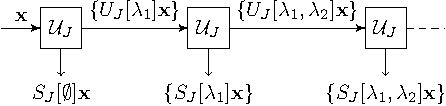
\includegraphics[width=3.3in, height=2in, keepaspectratio]{scatnet_crop.pdf}
        \caption[Scattering convolution network.]{\centering  Scattering networks can be seen as neural networks iterating over wavelet  modulus  operators $\mcalU_{J}$. Each layer $m$ outputs the averaged  invariants $S[p_{m}]\bfx$ and covariant coefficients $U[p_{m+1}]\bfx$.}
        \label{fig:SCN 1}
        % TODO: Change it for something similar to Siffre rigid motion
      \end{center}
      \vspace{-15pt}
    \end{figure}
    
    The scattering energy is mainly concentrated along frequency decreasing paths, \ie for which $\abs{\lambda_{k+1}} \leq \abs{\lambda_{k}}$~\cite{mallat2012gis}. The energy contained in the other paths is negligible and thus for applications only frequency decreasing paths are considered. Moreover there exists a path length $M > 0$ after which all longer paths can be neglected. For signal processing applications, this decay appears to be exponential and for classification applications, paths of length $M = 3$, \ie two convolutions, provide the most interesting results~\cite{anden2011multiscale, bruna2010classification}.
      
    This restrictions yield a more convenient parametrization of a scattering network. Indeed its now completely defined by the mother wavelet $\phi$, the maximum path length considered $M$, the finest scale level considered $J$, and the number of orientation considered $L$.
      
    Hence for a given set of parameters $(\psi, M,J,L)$, let $ST_{(\psi,M,J,L)}(\bfx)$ denote the unique frequency decreasing windowed scattering convolutional network with those parameters evaluated for signal $\bfx$. Each node $i$ of this network generates a, possibly empty, set of nodes $\{U_{(.)}, S_{(.)}\}$ of size $n_{i} = (j_{i}-1)L$ where $j_{i}$ is the scale of node $i$ and $L$ the number of orientations considered. SCN's architecture is displayed by Figure~\ref{fig:SCN 2}.

    \begin{figure}
      \begin{center}
        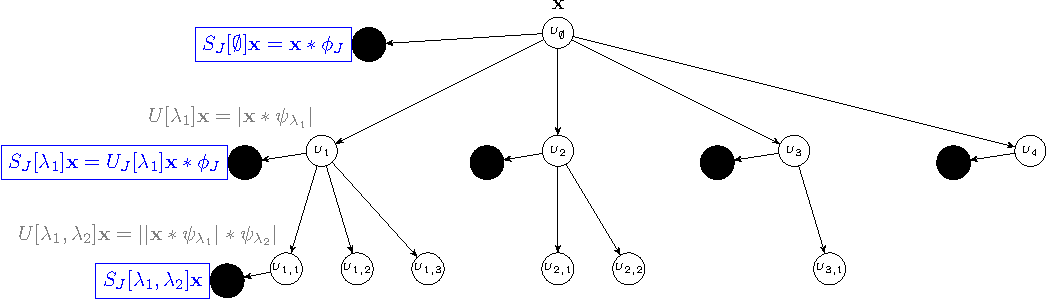
\includegraphics[width=3.3in, height=2in, keepaspectratio]{ST_freqDec_crop.pdf}
        \caption[Frequency decreasing scattering convolution network.]{\centering  Frequency decreasing scattering convolution network with $J=4$, $L=1$ and $M=2$. A node $i$ at scale $j_{i}$ generates $(j_{i}-1) \times L$ nodes. }
        \label{fig:SCN 2}
        % TODO: Narrow the gaps
      \end{center}
      \vspace{-15pt}
    \end{figure}
  
  \vspace{-5pt}
  \subsection{Scattering convolutional classifier}
    \label{subsec:SCN/SCC}
    \vspace{-5pt}
    In the original framework~\cite{bruna2013scattering}, the scattering network $ST_{(\psi, M,J,L)}(.)$ is used for a classification task using a SVM classifier on the outputs of the network. Performance can be slightly improved by adding a feature selection step to perform PCA on the scattering coefficients and keep only the most informative ones. This classification framework provides
    results comparable with the state of the art on several datasets~\cite{bruna2010classification}.


\section{The Scattering hidden Markov tree}
  \label{sec:SCHMT}
  \vspace{-5pt}
  State of the art performance can be achieved using SCNs associated with SVMs. However this approach is not adapted to very small training sets; nor does it deliver a probabilistic output. To overcome these
  limitations we propose an adaptation of the Crouse~\cite{crouse1998wavelet} and Durand~\cite{durand2004computational} wavelet hidden Markov trees to the non-regular, non-homogeneous tree structure of SCNs.
  
  \vspace{-5pt}
  \subsection{Hidden Markov tree model}
    \label{subsec:SCHMT/HMT model}
    \vspace{-5pt}
    The HMT models the marginal distribution of each real scattering coefficient $S_i$ as a Gaussian mixture. To each $S_i$, we associate a discrete hidden state $H_i$ that takes on values in $\llbracket 1,K \rrbracket$ with probability mass function $P(H_i)$. Conditioned on $H_i = k$, $S_i$ is Gaussian with mean $\mu_{i,k}$ and variance $\sigma_{i,k}$. Thus, its overall marginal PDF is given by $P(w_i) = \sum_{k=1}^{K} P(H_i = k)P(S_i| H_i=k)$ with $P(S_i|H_i=k) \sim \mcalN(\mu_{i,k}, \sigma_{i,k})$. While each scattering coefficient $S_i$ is conditionally Gaussian given its state variable $H_i$, overall it has a non-Gaussian density. Finally the probability for the hidden node $H_{i}$ to be in state $k$ given its father's state $g$ is characterized by a transition probability such that $\epsilon_{i}^{(gk)} = P(H_{i}= k | H_{\rho(i)}=g)$. This yields $P(H_{i}=k) = \sum_{g=1}^{K} \epsilon_{i}^{(gk)} P(H_{\rho(i)}=g)$.

    Such a model is pictured in Figure~\ref{fig:SCHMT 1} and for a given scattering architecture ---\ie fixed $M$, $J$ and $L$--- the SCHMT model is fully parametrized by,
    \vspace{-5pt}
    \begin{equation}
      \Theta = \big(\pi_{0}, \{ \epsilon_{i}, \{ \theta_{k,i} \}_{k\in\llbracket1,K\rrbracket} \}_{i\in\mcalT}\big).
      \label{eq:SCHMT - parameters}
    \end{equation}
    \vspace{-15pt}

    \begin{figure}
      \begin{center}
        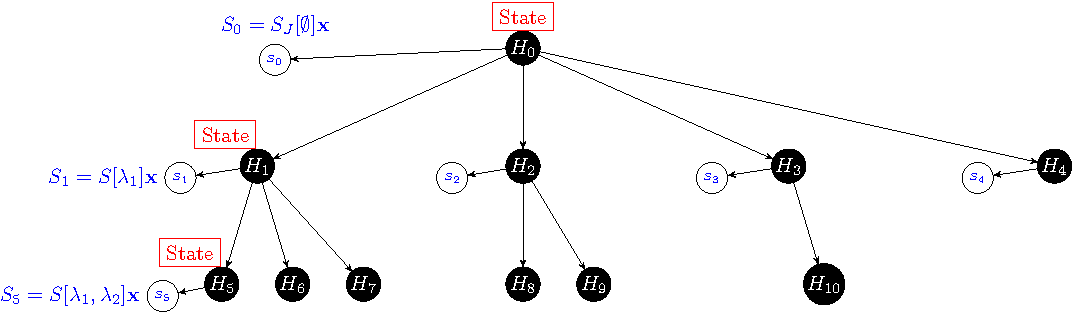
\includegraphics[width=3.3in, height=2in, keepaspectratio]{scat_HMT_crop.pdf}
        \caption{Scattering convolutional hidden Markov tree.}
        \label{fig:SCHMT 1}
        % TODO: Narrow the gaps
      \end{center}
      \vspace{-15pt}
    \end{figure}
    
    This model implies two assumptions on the scattering transform.  We firstly posit $K$-populations; i.e. that each scattering coefficient of a given signal can be described by $K$ clusters. This is a common assumption for standard wavelets~\cite{kingsbury2001complex} and it can hence be extended to the scattering transform. The SCHMT also assumes persistence in that the informative character of a
    coefficient is propagated across layers. This assumption is justified by the fact that scattering coefficients are highly correlated~\cite{oyallon2014deep}.
  
  \vspace{-5pt}
  \subsection{Learning the tree parameters}
    \label{subsec:SCHMT/Learning}    
    \vspace{-5pt}
    The proposed SCHMT is trained using the smoothed version of the Expectation-Maximization (EM) algorithm for hidden Markov trees proposed by Durand~\cite{durand2001statistical} and adapted to non-homogeneous and non-binary trees.
    
    Let $\bar{\mcalS}_{i}= \bar{s}_{i}$ be the observed sub-tree rooted at node $i$. By convention $\bar{\mcalS}_{0}$ denotes the entire observed tree. The smoothed version of the E-step requires the computation of the conditional probability distributions $\xi_{i}(k) = P(H_{i}=k | \bar{\mcalS}_{i}= \bar{s}_{i})$ (smoothed probability) and $P(H_{i}=k, H_{\rho(i)}=g | \bar{\mcalS}_{i}= \bar{s}_{i})$ for each node $i$ of the tree $\mcalT$ and states $k$ and $g$. This can be achieved through an upward-downward recursion displayed in Algorithm~\ref{algo:Smoothed upward} and~\ref{algo:Smoothed downward}. The output from the downward step are used in the M-step as shown in Algorithm~\ref{algo:Mstep}.
    
    \vspace{-15pt}
    \setlength{\algomargin}{+4pt}
    \begin{center}
      \begin{algorithm}
				\vspace{-3pt}
				\fontsize{8pt}{10pt}\selectfont
%          \textbf{Meta-parameters:}\\
%         $K$\\
        \tcp{Initialization:}
%         \tcp{$P_{\theta_{k,i}}(s_{i})$:}
        \For{All the nodes $i$ of the tree $\mcalT$}{ 
          $P_{\theta_{k,i}}(s_{i}) = \mcalN(s_{i} | \mu_{k,i},\sigma_{k,i})$
        }
%         \tcp{Loop over the leaves $i$ of the tree:}
        \For{All the leaves $i$ of the tree $\mcalT$}{
          $\beta_{i}(k) = \frac{P_{\theta_{k,i}}(s_{i}) P(H_{i}=k)}{\sum_{g=1}^{K} P_{\theta_{g,i}}(s_{i}) P(H_{i}=g)}$\\
          $\beta_{i,\rho(i)}(k) = \sum_{g=1}^{K}\frac{\beta_{i}(g) \epsilon_{i}^{(kg)}}{P(H_{i}=g)} . P(H_{\rho(i)}=k)$ \\
          $l_{i} = 0$
        }
        \tcp{Induction:}
%         \tcp{Bottom-Up loop over the nodes of the tree:}
        \For{All non-leaf nodes $i$ of the tree $\mcalT$ (Bottom-up)}{
          $M_{i} = \sum_{k=1}^{K} P_{\theta_{k,i}}(s_{i}) \prod_{j \in c(i)} \frac{\beta_{j,i}(k)}{P(H_{i}=k)^{n_{i}-1}}$ \\
          $l_{i} = \log(M_{i}) + \sum_{j \in c(i)}l_{j}$\\
          $\beta_{i}(k) = \frac{P_{\theta_{k,i}(s_{i})} \prod_{j \in c(i)}(\beta_{j,i}(k))}{P(H_{i}=k) ^{n_{i}-1} M_{i}} $\\
          \For{All the children nodes $j$ of node $i$}{
            $\beta_{i\backslash c(i)}(k) = \frac{\beta_{i}(k)}{\beta_{i,j}(k)}$
          }
          $\beta_{i,\rho(i)}(k) = \sum_{g=1}^{K} \frac{\beta_{i}(g) \epsilon_{i}^{(kg)}}{P(H_{i}=g)} .P(H_{\rho(i)}=k)$
        }
        \caption{Smoothed upward algorithm.}
        \label{algo:Smoothed upward}
        \vspace{-5pt}
      \end{algorithm}        
    \end{center}
    \vspace{-30pt}
    \vspace{-20pt}  
    \begin{center}
      \begin{algorithm}
				\vspace{-3pt}
				\fontsize{8pt}{10pt}\selectfont
%         \textbf{Meta-parameters:}\\
%         $K$\\
        \tcp{Initialization:}
        $\alpha_{0}(k) = 1$\\
        \tcp{Induction:}
%         \tcp{Top-Down loop over the nodes of the tree:}
        \For{All nodes $i$ of the tree $\mcalT\backslash\{0\}$ (Top-Down)}{
          $\alpha_{i}(k) = \frac{1}{P(H_{i}=k)} \sum_{g=1}^{K} \alpha_{\rho(i)}(g) \epsilon_{i}^{(gk)} \beta_{\rho(i)\backslash i}(g) P(H_{\rho(i)}=g)$
        }
        \caption{Smoothed downward algorithm.}
        \label{algo:Smoothed downward}  
				\vspace{-5pt}
      \end{algorithm}        
    \end{center}
    \vspace{-30pt}
    \vspace{-20pt}  
    \begin{center}
      \begin{algorithm}
			\vspace{-3pt}
			\fontsize{8pt}{10pt}\selectfont
%         \textbf{Meta-parameters:}\\
%         $K$,\\
%         Distribution family for $P_{\theta}$ \tcp*{Here Gaussian}
%         $N$ \tcp*{Number of observed realizations of the signal}
        \tcp{Initialization:}
        $\pi_{0}(k) = \frac{1}{N} \sum_{n=1}^{N} P(H_{0}^{n}=m|s_{0}^{n},\Theta^{l})$\\
        \tcp{Induction:}
%         \tcp{Loop over the nodes of the tree:}
        \For{All nodes $i$ of the tree $\mcalT\backslash\{0\}$}{
          $P(H_{i}=k) = \frac{1}{N} \sum_{n=1}^{N} P(H_{i}^{n}=k|\bar{s}_{0}^{n},\Theta^{l})$,\\
          $\epsilon_{i}^{gk} = \frac{\sum_{n=1}^{N} P(H_{i}^{n} = k, H_{\rho(i)}^{n}=g |\bar{s}_{0}^{n}, \Theta^{l})} {N P(H_{\rho(i)}=k)}$,\\
          $\mu_{k,i} = \frac{\sum_{n=1}^{N} s_{i}^{n} P(H_{i}^{n} = k |\bar{s}_{0}^{n}, \Theta^{l})} {N P(H_{i}=k)}$,\\
          $\sigma_{k,i}^{2} = \frac{\sum_{n=1}^{N} (s_{i}^{n} - \mu_{k,i})^{2} P(H_{i}^{n} = k |\bar{s}_{0}^{n}, \Theta^{l})} {N P(H_{i}=k)}$.
        }
        \caption{M-step of the EM algorithm.}
        \label{algo:Mstep}
				\vspace{-5pt}
      \end{algorithm}        
    \end{center}
    \vspace{-40pt}
   
  \vspace{-5pt}
	\subsection{MAP classification}
    \label{subsec:SCN/MAP}
    \vspace{-5pt}
    Let $\Theta_{c}$ now be a set of parameters for an SCHMT $\mcalT$ learned on a training set $\{\bar{S}_{0,c}^n\}_{n \in \llbracket1, N \rrbracket} = \{ST_{(\psi, J, M, L)}(\bfx_{c}^{n})\}_{n \in \llbracket1, N \rrbracket}$ composed of the scattering representations of $N$ realizations of a signal of class $c$ . Let also $\bfx^{new}$ be another realization of this signal, not used for training and $\mcalT^{new}$ be the instance of the SCHMT generated by this realization.

    In this context the MAP algorithm~\cite{durand2001statistical} aims to find the optimal hidden tree $\hat{\bar{h}}_{0}^{new}=(\hat{h}_{0}^{new}, \ldots , \hat{h}_{I-1}^{new})$ that maximizes the probability of this sequence given the model's parameters $P(\bar{\mcalH}_{0}= \hat{\bar{h}}_{0}^{new}|\mcalT^{new},\Theta_{c})$. The MAP framework also provides $\hat{P}$ the value of this maximum.
    
\section{Experiments}
  \label{sec:Exps}
  \vspace{-5pt}
  We compare the performance of SCHMT to those of a SCN combined with an SVM (SCN+SVM) restricted to a small number of training examples by performing two experiments on the digit classification dataset MNIST~\cite{lecun2016web}. It contains $60000$ training examples and $10000$ test images of $10$ handwritten digits (zero to nine), with $28\times28$ pixels.
  For both experiments we use a scattering transform with $M=3$ orders, $J=3$ scales, $L=3$ orientations and a Morlet mother wavelet. The hidden Markov tree has $K=2$ states and uses a mixture of Gaussian to describe the relationship between the scattering coefficients and the hidden states. For the SVM, the best parameters are selected by cross-validation.
  
  \vspace{-5pt}
  \subsection{MNIST - ``One vs All''}
		\label{subsec:Exps/MNIST - 1vsAll}
		\vspace{-5pt}
		In a similar fashion to~\cite{salakhutdinov2010one}, we first test SCHMT on a ``One vs All'' basis. However we propose this experiment with a more challenging setup. Indeed they pretrain their model with $100$ samples from each class but one. They then provide only limited amount of training examples, say $N$, for this last class. Instead we propose a framework where all the classes have the same limited amount of training points $N$. We then test the models on $1000$ examples.
		
		Table~\ref{tab:Exp1 results} displays the accuracy and the sensitivity for both SCHMTs and SCN+SVMs. With $N=5$ training examples, SVM is not able to discriminate the digit of interest and simply classify everything as ``All''. This yields a sensitivity of $0.0\%$ characteristic of an uninformative test. In the same condition, SCHMT is able to correctly discriminate the digit of interest and provides a very informative test --good sensitivity and accuracy. Some classes ---$4$ and $6$--- are more challenging than others due to their high intra-class variability.
		
    
    %Note that this experimental setup should be in favor of the SVM classifier since it is effectively provided with $9N$ training points for one class. With this amount training samples,
    \begin{figure}
      \hspace{35pt}
      \begin{tabular}{  |p{0.9cm}
                         p{0.7cm}
                        |p{1.1cm}
                        |p{1.5cm}|}
        \hline
        \multicolumn{2}{|c|}{\multirow{2}{*}{\parbox[t]{2cm}{1 vs All class}}} & \multicolumn{2}{c|}{MNIST}\\
        \cline{3-4}
                                      &   & SCHMT   & SCN+SVM \\
        \hline
        \multirow{2}{0pt}{$9$}        & (Acc) & $\mathbf{97.2\%}$ & $90.0\%$ \\
        \cdashline{3-4}
                                      & (Sen) & $\mathbf{94.0\%}$ & $0.0\%$ \\
                                      %& (PTR)   & $\mathbf{3.8}$     & $0$   \\
        \hline
        \multirow{2}{0pt}{$6$}        & (Acc) & $\mathbf{94.1\%}$ & $90.0\%$ \\
        \cdashline{3-4}
                                      & (Sen) & $\mathbf{57.5\%}$ & $0.0\%$ \\
                                      %&  (PTR) & $\mathbf{30.7}$    & $0$   \\
        \hline
        \multirow{2}{0pt}{Average}    & (Acc) & $\mathbf{93.9\%}$ & $90.0\%$ \\
        \cdashline{3-4}
                                      & (Sen) & $\mathbf{60.2\%}$ & $0.0\%$ \\
                                      %& (PTR)   & $\mathbf{75.5}$    & $0$    \\
        \hline
      \end{tabular}
      \caption{Accuracy and sensitivity on $1000$ samples of MNIST trained using only a $5$ of training points per class and tested on ``One vs All''.}
      \label{tab:Exp1 results}
      \vspace{-15pt}
    \end{figure}

  \vspace{-5pt}
  \subsection{MNIST - Full}
    \label{subsec:Exps/MNIST - Full}
    \vspace{-5pt}
		SCHMT and SCN+SVM are tested on the more complex problem of mutliclass labelling. SCHMT and SCN+SVM are both trained on a limited number of training examples per class and tested on the full testset.

		\begin{figure}
      \hspace{40pt}
      \begin{tabular}{  |p{2.5cm}
                        |p{1.5cm}
                        |p{1.5cm}|}
        \hline
        \multirow{2}{*}{\parbox[t]{2.5cm}{Training samples \\ per class}} & \multicolumn{2}{c|}{MNIST}\\
        \cline{2-3}
                & SCHMT & SCN+SVM \\
        \hline
        $N = 2$     & $\mathbf{28.6}\%$  & $18.7\%$   \\
        \hline
        $N = 5$     & $\mathbf{48.0\%}$ & $43.2\%$  \\
        \hline
        $N = 10$    & $45.2\%$  & $\mathbf{49.9\%}$  \\       
        \hline
      \end{tabular}
      \caption{Classification score on the complete testset of MNIST ($10000$ samples) trained using only a limited number $N$ of training points per class}
      \label{tab:Exp2 results}
      \vspace{-15pt}
    \end{figure}
		
    The best results for each models are displayed in Table~\ref{tab:Exp2 results}. SCHMT displays better generalization and prediction properties than SCN+SVM when trained on a very limited number of training points. For $N=2$ seen samples per class, SVM beats a random selector---\ie $10\%$--- by a small margin while SCHMT provides a near three folds improvement. With only $5$ training examples per class, SCHMT does close to five times better than random. As expected, when the number of training samples grow large enough ---\ie $10$ and more, SCN+SVM reaches better maximum classification score.
		
		The drop in performance of SCHMT for $N=10$ training examples is explained by the fact that the EM algorithm is undermined by convergence to local minima issues~\cite{moon1996expectation} yielding sometimes to poor learning quality for SCHMTs. However when a good minima is found, SCHMTs has acceptable generalization performance. 
    
    While confirming the superiority of our model in terms of generalizability for limited number of training points, this experiment also highlights a potential weakness of it in that sometimes convergence problems occur. However, in the main, SCHMT provides good classification score for such a low number of training examples.
		
\section{Conclusion}
  \label{sec:Conclusion}
  \vspace{-5pt}
  A SCHMT framework has been proposed which comprises a scattering transform and a hidden Markov tree model.  The scattering transform projects the data into a representational space of even higher dimensionality but of reduced volume along the invariants in the data. Then a probabilistic graphical model ---hidden Markov tree--- was used to fit a generative model to the distribution of the representation of the data.  As such, the proposed model takes advantage of the way in which the scattering transform introduces invariances into the representation but also the manner in which hidden Markov models capture dependencies between coefficients.  Experiments have demonstrated that the modelled distribution can be used to perform efficient classification tasks even with small training sizes. Even though we only here consider classification, a generative model is much more versatile than a simple ---yet efficient--- discriminative one. Because they model the full distribution of the data they can express more complex relationships between the observed and the unknown variables than simple discrimination. 
  
  To enhance SCHMT and especially the chance of converging toward a good minima during the EM learning, further work will include development of variational methodology to learn the model parameters~\cite{wainwright2008graphical}.

  
% To start a new column (but not a new page) and help balance the last-page
% column length use \vfill\pagebreak.
% -------------------------------------------------------------------------
\vfill
\pagebreak

% \section{COPYRIGHT FORMS}
% \l1abel{sec:copyright}
% 
% You must include your fully completed, signed IEEE copyright release form when
% form when you submit your paper. We {\bf must} have this form before your paper
% can be published in the proceedings.

% \section{REFERENCES}
% \label{sec:ref}
% References should be produced using the bibtex program from suitable
% BiBTeX files (here: strings, refs, manuals). The IEEEbib.bst bibliography
% style file from IEEE produces unsorted bibliography list.
% -------------------------------------------------------------------------
\bibliographystyle{IEEEbib}
\bibliography{strings}

% \bibliography{bib_icip}

\end{document}
